%% grundlagen.tex
%% $Id: grundlagen.tex 28 2007-01-18 16:31:32Z bless $
%%

\chapter{Related Work}
\label{ch:RelatedWork}

A project which also uses HTML/XHTML to make documents accessible is discussed in a paper \cite{markdownSyntax} by Voegler et al.. HTML is chosen as a book format, because it is operating system independent, accessible to screen readers and the content can be adapted visually to a person's wishes.  However, the work is generally not done by the original document author. Instead university/service staff or students transcribe it to accessible versions. They have to request the content from authors and get permission. 
Coding with HTML creates problems like linking errors, invalid HTML-code, etc., so Voegler et al. recommend using Markdown \cite{Markdown}, which is easier to write than HTML. It can then be converted to a variety of formats using pandoc \cite{Pandoc}, which also converts LaTeX code to MathML.
While reducing the number of mistakes compared to HTML, Markdown still requires programming and only people with sufficient knowledge of it will be able to use it effectively. Students doing the transcription will be more knowledgeable in coding than teachers in schools for the blind. 

If EPUB is compared to HTML as a book format, it is of course very similar as EPUB uses HTML/XHTML. HTML as a book format can be described as a simplified version of EPUB only without the packaging such as the package document, in essence only having the OEBPS folder. However, images have to be added manually to the folders, and CSS files have to be created. These are extra steps that might result in frequent mistakes. Furthermore, pandoc is command line based and is therefore more difficult to use than programs with a graphical user interface (GUI). It also has to be run separately after coding in Markdown, instead of being integrated in the creation process. Nevertheless, this paper shows that HTML, if created properly, is suitable to the needs of blind and visually impaired students.

Another approach is offered by Leporini et al. in their project Book4All \cite{book4all}. It originally allowed PDFs to be exported to XHTML or DAISY and later EPUB 3 was added as an option. It reads the PDF with the internal PDF Viewer to gather information about fonts and recognize if the document is in a multi-column layout. Then Book4All has to take this information and extracts the text and semantic information. This includes keeping the format of the PDF, such as recognizing headings, images and tables and adding appropriate tags to them. The user has the option of correcting tagging mistakes. It then has to be exported to its final format. 

\begin{figure}[H]
	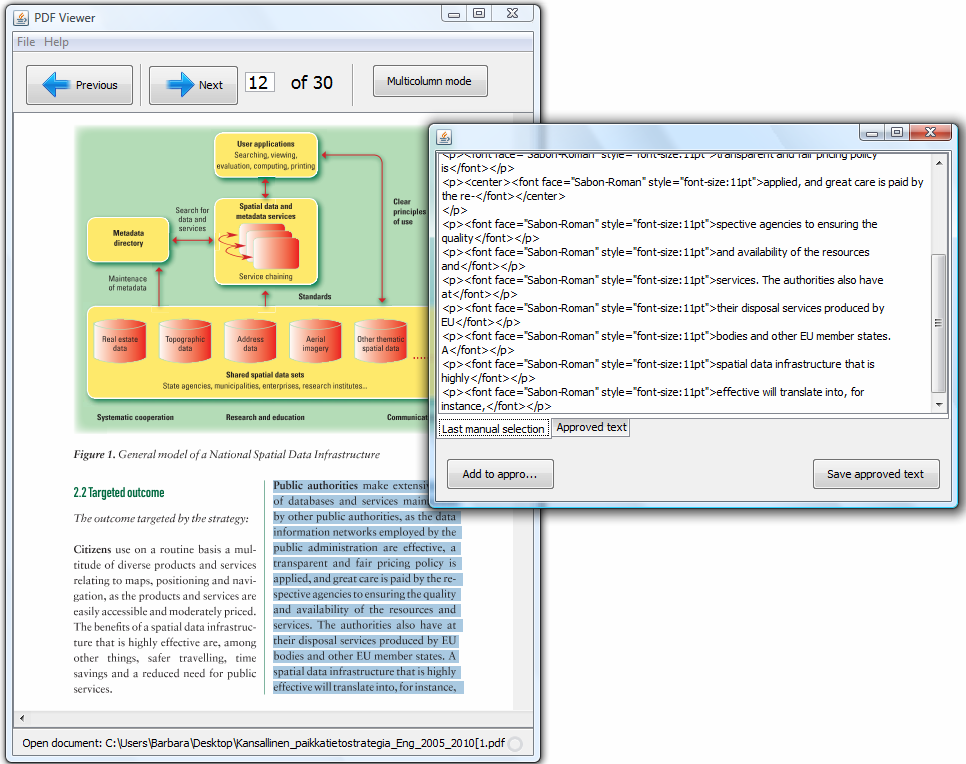
\includegraphics[width=\linewidth]{figures/book4all1.png}
	\caption{A view of the ad-hoc PDF Viewer extracting text from a multi-column layout document \protect\cite{book4all}}
	\label{fig:book4all1}
\end{figure}

Book4All attempts to semi-automate the conversion process as far as possible, but still offers the option of post processing the resulting markup as shown in figure~\ref{fig:book4all1}. While this is optional, important parts like alternative text for images can only be added like this. The markup is in Intermediate Book Format (IBF), which is based on XML. Without basic knowledge of XML, post-processing becomes much more difficult. 

\begin{figure}[H]
	\centering
	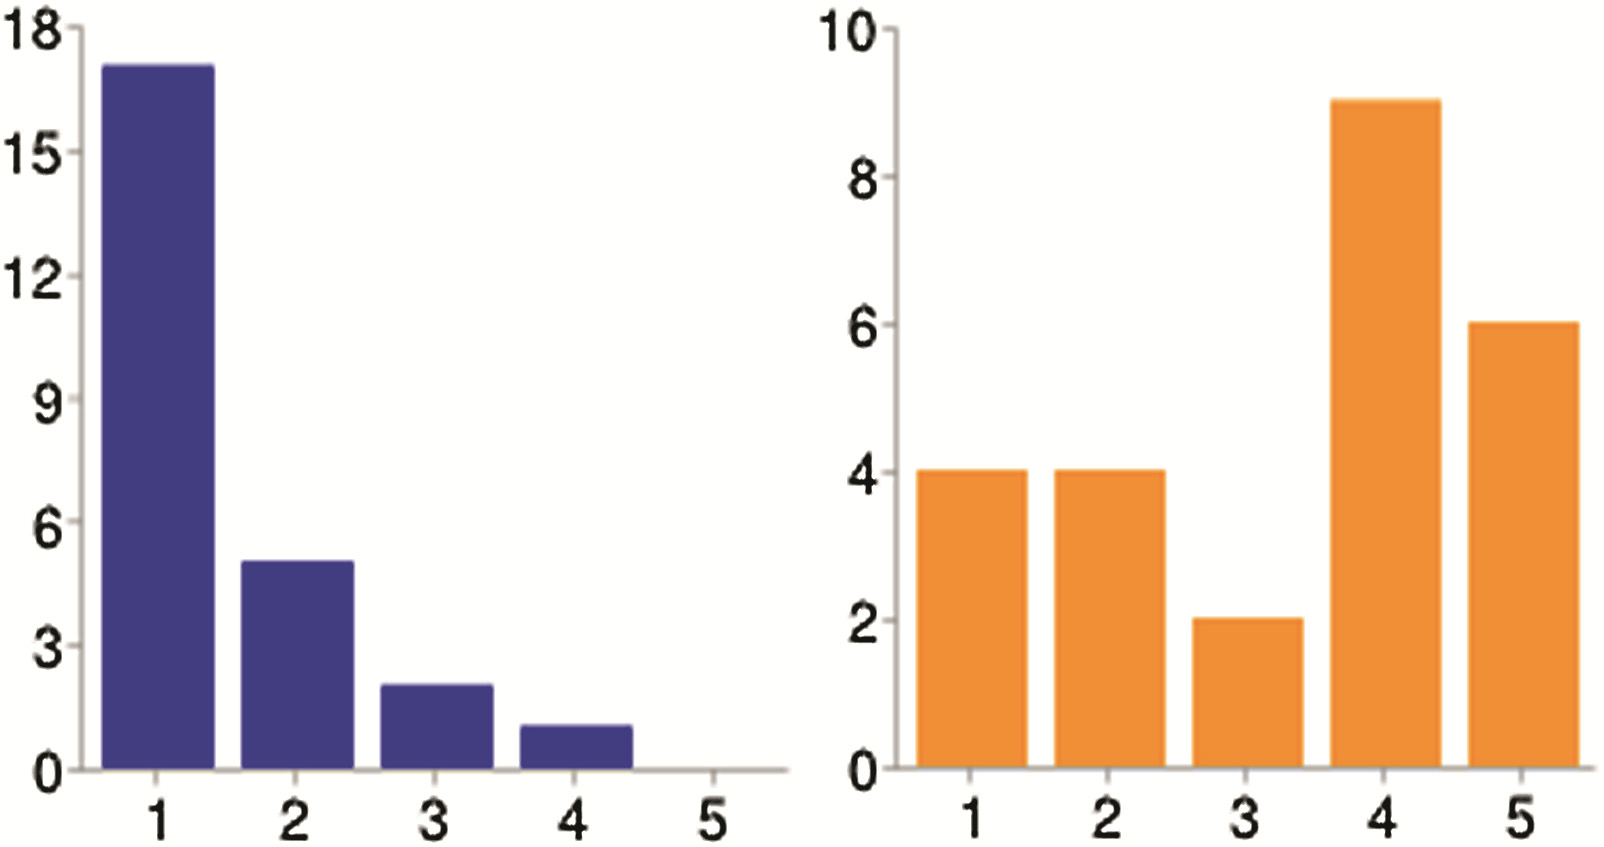
\includegraphics[width=\linewidth*4/5]{figures/easeOfContentAccess.png}
	\caption{Difficulty degree to access the content for the EPUB (blue, left) and PDF (orange, right), respectively (1-not difficult
		to 5-very difficult) \protect\cite{enrichEPUB}} 
	\label{fig:enrichEpub1}
\end{figure}

Bartalesi and Leporini \cite{enrichEPUB} also carried out an online survey in a follow-up work and asked 25 users to rate "enriched" EPUBs created in Book4All in comparison to the original PDF format regarding accessibility and usability. $50\%$ of respondents preferred EPUB over other e-book formats, while $13\%$ said EPUB was equivalent.
The sample group also felt that it was easier to access content in EPUBs and use the table of contents than in PDFs.
Furthermore, $80\%$ of blind users were unable to read images in PDFs correctly with their screen reader, while the corresponding value for EPUBs was less than $50\%$. $64\%$ of users found the EPUB's document structure easy to understand. Users also reported that it is much easier to access content in the EPUB than in a PDF, as shown in figure~\ref{fig:enrichEpub1}.  The results show that EPUB is a suitable format for blind people, if the EPUB contains proper tagging. 
These works motivate us to develop a new universal approach.

